% در این قسمت نحوه‌ی نصب DoxyGen روی سیستم عامل ویندوز توضیح داده شده است.
% محمد هادی منصوری. ۹۰/۳/۱
%
% حق نشر 1390-1402 دانش پژوهان ققنوس
% حقوق این اثر محفوظ است.
% 
% استفاده مجدد از متن و یا نتایج این اثر در هر شکل غیر قانونی است مگر اینکه متن حق
% نشر بالا در ابتدای تمامی مستندهای و یا برنامه‌های به دست آمده از این اثر
% بازنویسی شود. این کار باید برای تمامی مستندها، متنهای تبلیغاتی برنامه‌های
% کاربردی و سایر مواردی که از این اثر به دست می‌آید مندرج شده و در قسمت تقدیر از
% صاحب این اثر نام برده شود.
% 
% نام گروه دانش پژوهان ققنوس ممکن است در محصولات دست آمده شده از این اثر درج
% نشود که در این حالت با مطالبی که در بالا اورده شده در تضاد نیست. برای اطلاع
% بیشتر در مورد حق نشر آدرس زیر مراجعه کنید:
% 
% http://dpq.co.ir/licence
%
\section{ویندوز}

در آدرس
\url{http://www.doxygen.org/download.html} 
یک برنامه‌ی اجرایی برای نصب نسخه‌ی ویندوزی وجود دارد. این برنامه به صورت یک
مجموعه کامل قابل نصب است و نصب آن بسیار ساده است.
کافی است پنجره‌های محاوره‌ای را دنبال کنید.



در هنگام نصب در یکی از مراحل از کاربر خواسته می‌شود موارد لازم برای نصب را تعیین کند. 
تصویر \ref{پنجره_نصب_روی_ویندوز} را ببینید. در این مرحله 
فهرستی از ابزارهایی که نصب می‌شودقرار داده شده است. 
همانگونه که در تصویر \ref{پنجره_نصب_روی_ویندوز} دیده می‌شود یکی از ابزارها، \lr{Doxywizard} است. 
به این ترتیب می‌توان در نسخه‌ی ویندوزی، هر دو ابزار \lr{Doxygen} و \lr{Doxywizard} را نصب کرد.

\begin{figure}
\centering
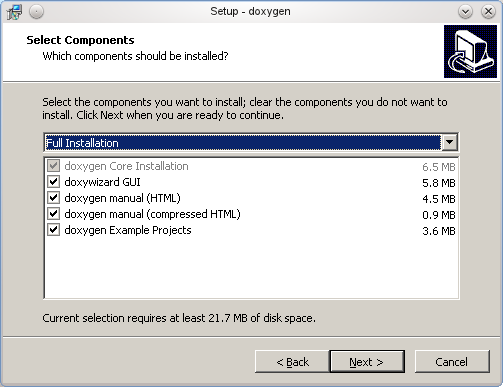
\includegraphics[width=0.75\textwidth]{image/windows_setup}
\caption[
پنجره‌ی محاوره‌ای نصب
{\lr{Doxygen}}
 روی ویندوز
]{
پنجره‌ی محاوره‌ای نصب
{\lr{Doxygen}}
 روی ویندوز. در این پنجره فهرستی از مواردی که باید نصب شود قرار دارد.
}
\label{پنجره_نصب_روی_ویندوز}
\end{figure}

توصیه می شود که بعد از نصب،
\lr{GraphViz} 
(نسخه‌ی ۲/۸ یا جدیدتر) را هم دریافت کرده و نصب کنید.
\lr{Doxygen}
 می تواند از ابزار
\lr{dot}
 مربوط به بسته‌ی
\lr{GraphViz}
، برای تولید بهتر دیاگرام ها استفاده کند.
% تنظیم \lr{HAVE\_DOT} در پرونده‌ی پیکربندی را مشاهده کنید.

اگر می‌خواهید پرونده‌های فشرده‌ی \lr{HTML} تولید کنید، نیاز به 
\lr{Microsoft HTML help} 
دارید. این ابزار را می‌توانید از آدرس 
\url{http://msdn.microsoft.com/en-us/library/ms670169}
 دریافت کنید.
%(تنظیم \lr{GENERATE\_HTMLHELP} را در پرونده‌ی پیکربندی مشاهده کنید)،

اگر می‌خواهید پرونده‌های فشرده‌ی \lr{Qt} را تولید کنید، نیاز به \lr{qhelpgenerator} دارید که قسمتی از \lr{Qt} 
 است. \lr{Qt} را می‌توانید از آدرس 
\url{http://qt.nokia.com/downloads/}
دریافت کنید.

به منظور تولید خروجی \lr{PDF}، یا استفاده از فرمول‌های خاص، احتیاج به نصب
\lr{LaTeX} و \lr{Ghostscript} دارید.
برای \lr{LaTex} چند توزیع وجود دارد. از جمله موارد معروف که باید با \lr{doxygen}
کار کنند \lr{MikTex} و \lr{XemTex} است\footnote{متاسفانه تولید مستند در قالب
\lr{LaTeX} با استفاده از \lr{Doxygen} برای مستندات به زبان فارسی با مشکلاتی
روبروست}.
\lr{Ghostscript} 
 را می‌توان از آدرس
\url{http://sourceforge.net/projects/ghostscript/} 
 دریافت کرد.

پس از نصب \lr{LaTex} و \lr{Ghostscript} باید مطمئن شوید که ابزارهای
\lr{latex.exe}، \lr{pdflatex.exe} و \lr{gswin32c.exe} در مسیر جستجوی دستورات خط
فرمان قرار دارند. در صورتی که از این موضوع مطمئن نیستید دستورالعمل زیر را دنبال
کنید و دستورات را در خط فرمان اجرا کنید تا ببینید به درستی کار می‌کنند یا نه.

از صفحه‌ی اصلی ویندوز روی \lr{My Computer} کلیک راست کرده و گزینه‌ی
\lr{Properties} را انتخاب کنید.
 در پنجره‌ای که ظاهر می‌شود زبانه‌ی \lr{Advanced} را انتخاب کنید. سپس دکمه‌ی
 \lr{Environment Variables} را کلیک کنید.
 در پنجره‌ای که ظاهر می‌شود متغیر \lr{Path} را انتخاب کرده و دکمه‌ی \lr{Edit} را
 کلیک کنید.
 سپس مسیرهای مربوط به ابزارهای گفته شده را در صورتی که وجود نداشت، در این قسمت
 اضافه کنید.
 مسیرهای مختلف با استفاده از علامت نقطه ویرگول از هم جدا می‌شوند. مثلا
\lr{C:\textbackslash Program Files;C:\textbackslash Winnt;C:\textbackslash
Winnt\textbackslash System32}.

پس از انجام کارهای گفته شده نرم‌افزار \lr{Doxygen} نصب شده و آماده استفاده است.